\documentclass[border=2pt]{standalone}
\usepackage{tikz}
\usetikzlibrary{arrows.meta,shapes.misc}
\begin{document}
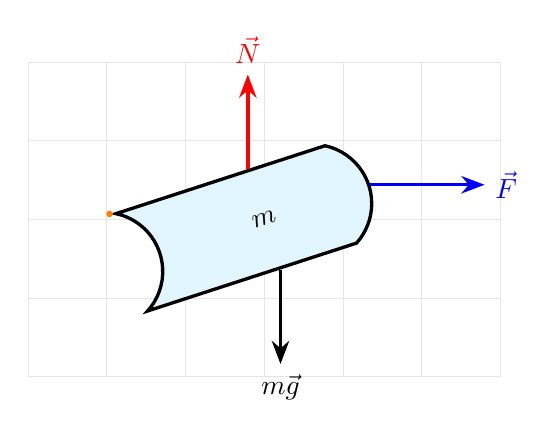
\begin{tikzpicture}[>=Stealth]
  \draw[step=1cm,gray!20,very thin] (-3,-2) grid (3,2);
  \node[rounded rectangle,draw,very thick,fill=cyan!12,
    rounded rectangle arc length=120,
    rounded rectangle west arc=concave,
    rounded rectangle east arc=convex,
    minimum width=34mm,minimum height=13mm,rotate=18] (body) at (0,0) {$m$};
  \draw[->,very thick,blue] (body.east) -- ++(1.45,0) node[right] {$\vec F$};
  \draw[->,very thick,red] (body.north) -- ++(0,1.2) node[above] {$\vec N$};
  \draw[->,very thick] (body.south) -- ++(0,-1.2) node[below] {$m\vec g$};
  \fill[orange] (body.north west) circle (1.2pt);
\end{tikzpicture}
\end{document}
